\documentclass[fleqn,12pt]{article}
\usepackage{amsmath}
\usepackage[colorlinks]{hyperref}
\usepackage{fullpage}
\setlength{\parindent}{0em}
\setlength{\parskip}{1em}
\usepackage{array}
\usepackage{tikz}
\usetikzlibrary{positioning}
\begin{document}
\thispagestyle{empty}

\section*{Logic pset 7}

Please answer \textbf{any three} of the following questions; each is
worth six points. Write your answers in your own words, making your
reasoning explicit. \textbf{Resource:} Chapter 8 of \textit{HLW}

\begin{enumerate}
\item Is there a valid proof with the following line fragments? Write
  your answer in the form of a short essay, using complete sentences.

  \begin{tabular}{>{\raggedleft\arraybackslash}p{1.5cm} >{\centering\arraybackslash}p{1.0cm} p{5cm} >{\raggedright\arraybackslash}p{3.5cm}}
    1 & (1) & $\exists x(Fx\to \forall yGy)$ & A \\
    \mbox{}  & \,\vdots & \\
    1 & (n) & $\exists xFx\to \forall yGy$ \end{tabular}

  No there is not. To see that the sentence on line 1 does not
  logicaly imply the sentence on line $n$, let $M$ be the model with
  domain $\{ \alpha ,\beta \}$ and where $F^M=\{ \alpha \}$ and
  $G^M=\emptyset$. The sentence on line 1 is true in $M$ because
  $\beta$ is in the extension of $Fx\to \forall yGy$. But the sentence
  on line $n$ is false in $M$ because $\exists xFx$ is true in $M$
  while $\forall yGy$ is false in $M$.

\item The sentence $P\to \exists xFx$ is not existential, and so is
  not a candidate for EE. But if there is a derivation of $\varphi$
  from $P\to Fa$ and auxiliary assumptions $\Delta$ that obeys the
  restrictions on EE (i.e.\ the name $a$ doesn't occur anywhere
  outside of the subproof), then is there also a derivation of
  $\varphi$ from $P\to \exists xFx$ and $\Delta$? Explain your answer.

  There are several ways to show that there is also a derivation of
  $\varphi$ from $P\to\exists xFx$ and $\Delta$. One simple way is to
  note that $P\to\exists xFx\vdash \exists x(P\to Fx)$. We assume that
  $\Delta ,\exists x(P\to Fx)\vdash \varphi$, and so the cut rule
  implies that $\Delta ,P\to \exists xFx\vdash \varphi$.

  In more prosaic terms, suppose that we have lines like this:

  \medskip \begin{tabular}{>{\raggedleft\arraybackslash}p{1.5cm}
     >{\centering\arraybackslash}p{1.0cm} p{5cm}
     >{\raggedright\arraybackslash}p{3.5cm}}
     $n_1$ & ($n_1$) & $P\to\exists xFx$ & A \\
    $n_2$ & ($n_2$) & $P\to Fa$ & A \end{tabular}
  
  \medskip Then we can continue the proof like this:

  \medskip \begin{tabular}{>{\raggedleft\arraybackslash}p{1.5cm}
     >{\centering\arraybackslash}p{1.0cm} p{5cm}
       >{\raggedright\arraybackslash}p{3.5cm}}
       $n_1$ & ($n_3$) & $\exists x(Fx\to P)$ \\
                & $\vdots$ & \\
       $\Delta ,n_2$ & ($n_4$) & $\varphi$ & (by assumption) \\
       $\Delta ,n_1$ & ($n_5$) & $\varphi$ & $n_3,n_2,n_4$ EE \end{tabular}
       
\item Consider the two sentences $\forall xFx\to P$ and
  $\forall x(Fx\to P)$, where $x$ does not occur in $P$. Are these
  sentences logically equivalent? Justify your answer by providing
  proofs and/or models. Write out your answer clearly enough that it
  would convince somebody who doesn't already get it.

  We can show $\forall x(Fx\to P)\vdash \forall xFx\to P$ by a proof,
  and we can show $\forall xFx\to P\not\vdash\forall x(Fx\to P)$ by
  giving a counterexample.

  Counterexample: let $M$ be the interpretation with domain
  $\{\alpha ,\beta\}$, where $F$ has extension $\{ \alpha \}$ and $P$
  is false. Then $\forall xFx\to P$ is true because $\forall xFx$ is
  false. But $\forall x(Fx\to P)$ is false because $\alpha$ is not in
  the extension of $Fx\to P$.

\item Consider the following two interpretations of the binary
  relation $R$, one with domain $\{ 1,2,3\}$ and the other with domain
  $\{ \alpha ,\beta ,\gamma \}$. Write a sentence that is true in one
  model but false in the other, and explain step by step how to
  determine its truth value in each. (Note that
  $1,2,3,\alpha ,\beta,\gamma$ are elements of the models; they are
  not names that can be used in your sentence.)

\begin{tabular}{cc}
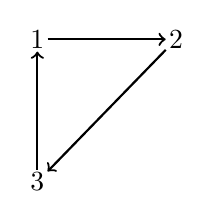
\begin{tikzpicture}[scale=1, every node/.style={inner sep=1pt, font=\normalsize}]
\node (a) {$1$};
\node[right=1.5cm of a] (b) {$2$};
\node[below=1.5cm of a] (c) {$3$};
\draw[->, thick] (a) -- (b);
\draw[->, thick] (b) -- (c);
\draw[->, thick] (c) -- (a);
\end{tikzpicture}

  &

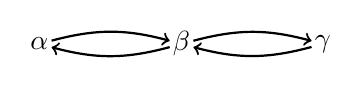
\begin{tikzpicture}[scale=1, every node/.style={inner sep=1pt, font=\normalsize}]
\node (a) {$\alpha$};
\node[right=1.5cm of a] (b) {$\beta$};
\node[right=1.5cm of b] (c) {$\gamma$};
% forward arrows
\draw[->, thick, bend left=15] (a) to (b);
\draw[->, thick, bend left=15] (b) to (c);
% backward arrows
\draw[->, thick, bend left=15] (b) to (a);
\draw[->, thick, bend left=15] (c) to (b);
\end{tikzpicture}    

\end{tabular}

Consider the sentence $\exists x\exists y(Rxy\wedge \neg Ryx)$. This
sentence is true in a model just in case there is a pair of elements
that fails to witness symmetry of $R$. Hence it is true in the first
model; in particular, $\langle 3,1\rangle$ is in the extension of $R$,
but $\langle 1,3\rangle$ is not in the extension of $R$. However, this
sentence is false in the second model since every arrow is matched by
an arrow in the opposite direction.


\item For each of the following sentences, provide one interpretation
  in which it is true and another in which it is false. An
  interpretation may be presented by giving a set $M$ and a subset
  $R^M$ of $M\times M$, or it may be presented as an arrow diagram. In
  either case, explain step-by-step how to determine the truth value
  of the sentence in the model.
  
  \begin{enumerate} \item $\forall x\forall y\exists z(Rxz\wedge Ryz)$

    Let the domain be $\{ \alpha \}$. If the extension of the relation
    $R$ is empty, then the extension of $Rxz\wedge Ryz$ is the empty
    subset of $M\times M\times M$, and so the truth-value of
    $\forall x\forall y\exists z(Rxz\wedge Ryz)$ if false.

    If, in contrast, the extension of the relation $R$ is
    $\{ \langle \alpha ,\alpha\rangle \}$, then the extension of
    $Rxz\wedge Ryz$ is $\{ \langle \alpha ,\alpha ,\alpha \}$. (Here
    we are adopting the convention that $x$ is the first coordinate,
    $y$ is the second, and $z$ is the third. Hence the extension of
    $\exists z(Rxz\wedge Ryz)$ is $\{ \langle\alpha
    ,\alpha\rangle\}$. But since
    $M\times M=\{ \langle \alpha ,\alpha\rangle \}$, it follows that
    $\forall x\forall y\exists z(Rxz\wedge Ryz)$ is true.
    
  \item $\forall x(\exists yRyx\to \forall zRzx)$

    This sentence effectively says that for every $x$, if there is an
    arrow coming into $x$ from some other node, then there must be an
    arrow coming into $x$ from every node. So one way to make it true
    is by having no arrows coming in from any nodes. In particular,
    let the domain be $\{ \alpha ,\beta \}$. If the extension of the
    relation $R$ is empty, then the extension of $\forall zRzx$ and
    $\exists yRyx$ are empty, hence the extension of
    $\exists yRyx\to \forall zRzx$ is $M$, and
    $\forall x(\exists yRyx\to \forall zRzx)$ is true.

    Now let the extension of the relation $R$ be
    $\{ \langle \alpha ,\alpha\rangle \}$. In this case, the extension
    of $\forall zRzx$ is empty, while the extension of $\exists yRyx$
    is $\{ \alpha \}$. Therefore the extension of
    $\exists yRyx\to \forall zRzx$ is $\{ \beta\}$. Since $\alpha$ is
    not in that set, it follows that
    $\forall x(\exists yRyx\to \forall zRzx)$ is false
\end{enumerate}





\end{enumerate}



\end{document}


%%% Local Variables:
%%% mode: latex
%%% TeX-master: t
%%% End:
